\documentclass[8 pt]{beamer}
\usepackage[utf8]{inputenc}
\usepackage{amsmath}
\usepackage{multirow}
\usepackage{cancel}
\usepackage{multicol}
\usepackage[document]{ragged2e}
\usepackage{hyperref}
\usepackage{xcolor}
\usepackage{color}
\usepackage{bm}
\usepackage{mathtools}
\definecolor{mygray}{gray}{0.7}

\usetheme{EastLansing}
%\usetheme{Pittsburgh}
%\usetheme[height=30pt]{Rochester}
%\usecolortheme{lily}
%\usecolortheme{spruce}

\newcommand{\backupbegin}{
   \newcounter{finalframe}
   \setcounter{finalframe}{\value{framenumber}}
}
\newcommand{\backupend}{
   \setcounter{framenumber}{\value{finalframe}}
}

% -- East Lansing --
\definecolor{mydarkgreen}{RGB}{0,81,40}
\definecolor{mymediumgreen}{RGB}{153, 193, 173}
\definecolor{mylightgreen}{RGB}{229, 239, 234}
\definecolor{mycolor}{RGB}{0,81,40}

\setbeamertemplate{blocks}[rounded][shadow=false]
\setbeamercolor{structure}{fg=mydarkgreen}
\setbeamercolor*{block title}{fg=mydarkgreen, bg=mymediumgreen}
\setbeamercolor*{block body}{fg=black, bg=mylightgreen}

% -- Pittsburgh
%\definecolor{mycolor}{RGB}{51,51,180} %Dark blue
%\definecolor{mycolor}{RGB}{192,57,43} %Dark red
%\definecolor{mycolor}{RGB}{0,81,40} %Dark green

%\setbeamercolor*{title}{use=structure,fg=mycolor,bg=mycolor!12}
%\setbeamertemplate{title page}[default][colsep=-4bp,rounded=true,shadow=false]

%\setbeamertemplate{frametitle}
%{
%	\begin{center}\color{mycolor}\textbf{\Large\insertframetitle}\end{center} \vspace{-5pt}
%}

%\setbeamercolor{structure}{fg=mycolor}
%\setbeamercolor{itemize item}{fg=black}

\setbeamertemplate{blocks}[rounded][shadow=false]
\setbeamercolor*{block title}{fg=mycolor, bg=mycolor!12}
\setbeamercolor*{block body}{fg=black, bg=mycolor!12}

\setbeamercolor*{block title example}{fg=mycolor, bg=mycolor!4}
\setbeamercolor*{block body example}{fg=mycolor, bg=mycolor!12}
\setbeamersize{text margin left=6mm,text margin right=6mm} 
  
%\addtobeamertemplate{navigation symbols}{}{%
%    \usebeamerfont{footline}%
%   \usebeamercolor[fg]{footline}%
%   \hspace{1em}%
%    \insertframenumber/\inserttotalframenumber
%}

\title{Statistical approach to muography}
\date{July 17th 2020}
\author{C\'{e}dric Prie\"els}

 \begin{document}


\begin{frame}
\vspace{-15pt} 
\title{Statistical approach to muography as a non-destructive \\ testing technique for industry problem solving}
\author{C\'{e}dric Prie\"els \\ \vspace{10pt} \textbf{Director} - Pablo Mart\'inez Ru\'iz del \'Arbol \newline \textbf{Co-director} - Carlos D\'iez \\ \vspace{20pt} 
\includegraphics[width= 0.15\textwidth]{figs/image_UC.png} \hspace{10pt} 
\includegraphics[width= 0.16\textwidth]{figs/muonSystems.png} \newline \vspace{20pt} Universidad de Cantabria \newline Muons systems \newline  \begin{center} \large{\textbf{July 17th 2020}} \end{center}}

\date{}
\vspace{15pt}
\maketitle

\centering
  
\end{frame}


\begin{frame}{Outline}

	\begin{itemize}
		\item Introduction \vfill
		\item Muons and muography \vfill
		\item Statistical basis of the algorithm
		\begin{itemize}
			\item Probability density functions
			\item Kernel density estimation
			\item Monte-Carlo simulations
			\item Likelihood minimization
		\end{itemize} \vfill
		\item The algorithm \vfill
		\item Results obtained \vfill
		\item Conclusions \vfill
	\end{itemize}

\end{frame}






%Introduction
\begin{frame}{}
	\centering
	\huge{\textbf{\color{mycolor} Section I}} \newline
	\LARGE{\textbf{\color{mycolor} General introduction \color{black}}} \vfill
	
	\LARGE{\textbf{\color{black} Main goal of this work \color{black}}}\newline \vspace{10pt} Develop a new framework allowing to perform a muography experiment to characterize the inner properties of physical objects using data science and advanced statistical models. \vfill
\end{frame}















%Theoretical introduction
\begin{frame}{Particle physics and muons}

\begin{minipage}[c]{.54\textwidth}
The Standard Model \textbf{describes the fundamental particles} existing and their interactions:
\begin{itemize}
	\justifying
	\item Introduced in the 1970s and still considered to be valid, but probably incomplete
	\item Simple in concept but extremely precise
	\item Lots of successful predictions made over the years, such as the existence of the top quark and the Higgs boson
\end{itemize}
\end{minipage} \hfill
\begin{minipage}[c]{.42\textwidth}
	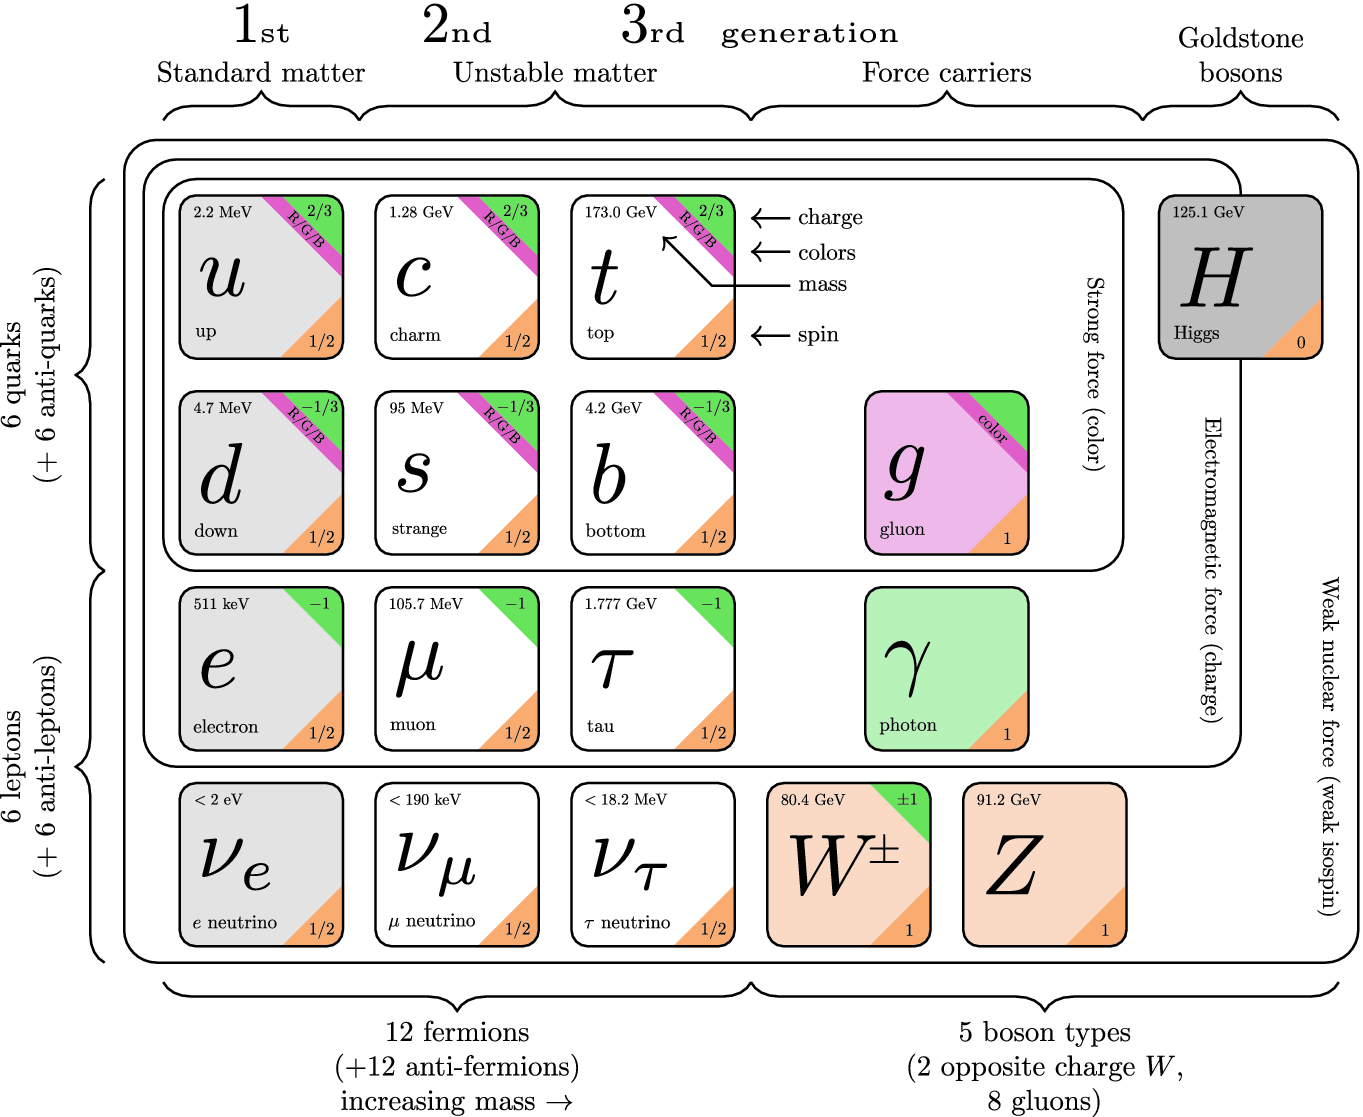
\includegraphics[width=5cm, height=4.2cm]{figs/SMFermions.png}
\end{minipage} \hfill \vfill

\begin{exampleblock}{} Muons \end{exampleblock}
\begin{itemize}
	\justifying
	\item Muons $\mu^-$ are one of the 12 fundamental particles existing
	\item They have a relatively small interaction cross-section with ordinary matter, allowing them to cross material without being stopped, making them interesting.
\end{itemize} \vfill
\end{frame}


\begin{frame}{Cosmic rays}
\justifying
Comic rays are a \textbf{constant flux of high energy particles} reaching the Earth:
\begin{itemize}
	\justifying
	\item Mostly made out of protons and atomic nuclei
	\item Trigger a decay chain by interacting with the atmosphere, producing muons
	\item Muons are not stable ($\tau \simeq 2.2\mu$s) but relativity can make them live long enough to reach the ground $\rightarrow$ 10.000 cosmic muons are observed per $m^2$ and per minute at sea level.
\end{itemize} \vfill

\begin{minipage}[c]{.98\textwidth}
	\begin{center}
	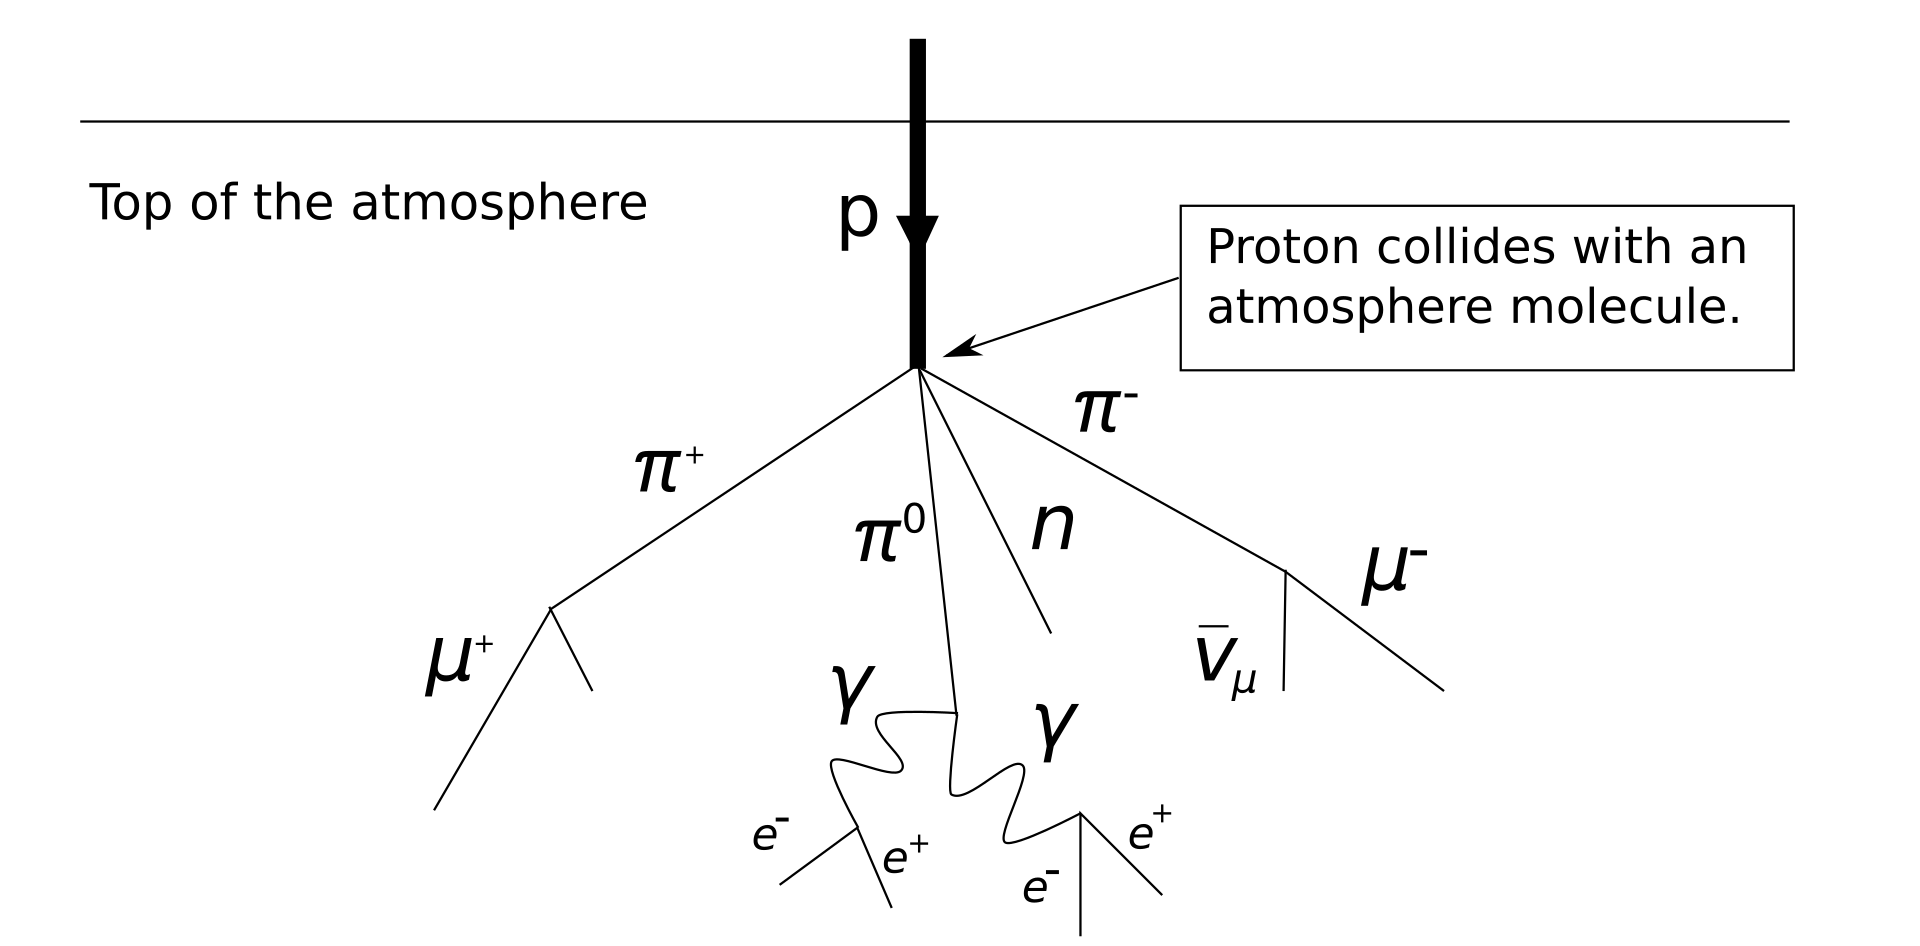
\includegraphics[width=8cm, height=4cm]{figs/cosmic.png}
	\end{center}
\end{minipage} \hfill \vfill
\end{frame}

\begin{frame}{Interaction with matter}
\justifying
Muons interact with matter through two main processes:
\begin{exampleblock}{} Ionization \end{exampleblock}
\textbf{Ionization}, when  the  incident  muon gives some of its energy to the electrons of the absorber, but quite small for MIPs such as cosmic muons. \\
\hspace{10pt} $\rightarrow$ Basis for the \textbf{\alert{absorption muography}}. \vfill

\begin{exampleblock}{} Multiple scattering \end{exampleblock}
\textbf{Multiple Coulomb scattering} inducing a \alert{\textbf{stochastic deviation}} whose central angular deviation can be described by a Gaussian of width $\theta_0$.

\begin{minipage}[c]{.48\textwidth}
\begin{equation*}
\label{eq:Moliere}
\theta_0 = \frac{13.6 \text{ MeV}}{\beta c p} \sqrt{\frac{x}{X_0}} \left [1 + 0.038 \ln \left (\frac{x}{X_0 \beta^2} \right ) \right ]
\end{equation*}

\justifying
This deviation depends on the number of radiation lengths $X_0$ and therefore on the medium crossed. \\
\hspace{10pt} $\rightarrow$ Basis for the \textbf{\alert{scattering muography}}.
\end{minipage} \hfill
\begin{minipage}[c]{.51\textwidth}
	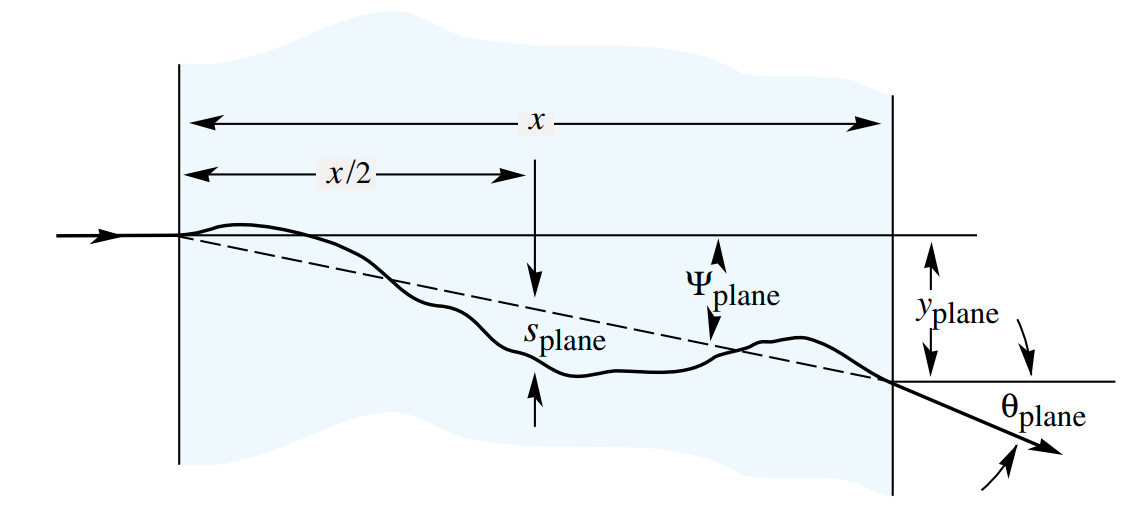
\includegraphics[width=6.3cm, height=2.6cm]{figs/moliere.png}
\end{minipage} \hfill \vfill
\end{frame}

\begin{frame}{Muon tomography}
Instead of \textit{calculating} the deviation expected for a cosmic muon, we can \textit{measure} the positional and angular deviation suffered \textbf{to estimate the properties of the medium crossed}. \\
\hspace{10pt} $\rightarrow$ Main idea behind the principle of \textbf{\alert{muon tomography}}, or \textbf{\alert{muography}}. \vfill


\begin{minipage}[c]{.49\textwidth}
\justifying
This method prevents several advantages over other imaging techniques:
\begin{itemize}
\justifying
\item Non-destructive technique
\item High penetrating capabilities allowing to probe large and dense objects
\item Completely safe, by using natural cosmic rays for the measurement.
\end{itemize} \vspace{10pt}

	Muography can be used in many different fields, for example to find hidden rooms in Pyramids or in volcanology to know whether a pocket is empty or full of lava [1].
\end{minipage} \hfill
\begin{minipage}[c]{.49\textwidth}
	\begin{center}
	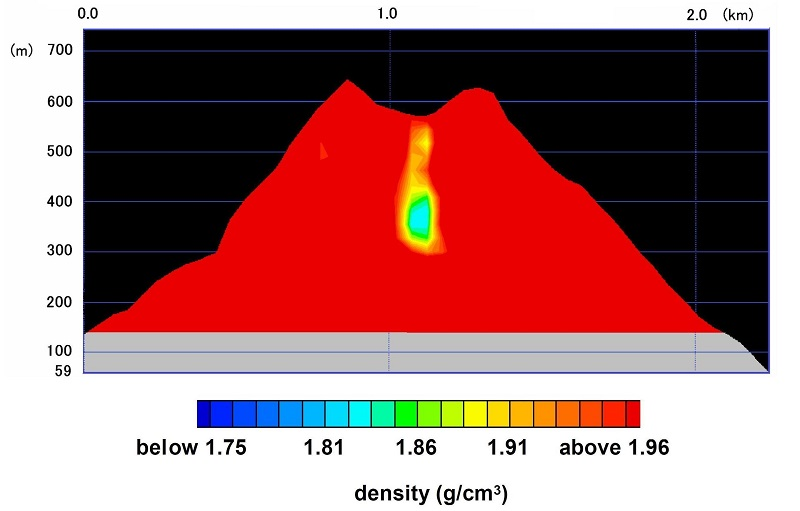
\includegraphics[width=6cm, height=4cm]{figs/volcano.jpg}
	\end{center}
\end{minipage} \hfill \vfill
\end{frame}

\begin{frame}{Experimental setup}
\begin{minipage}[c]{.50\textwidth}
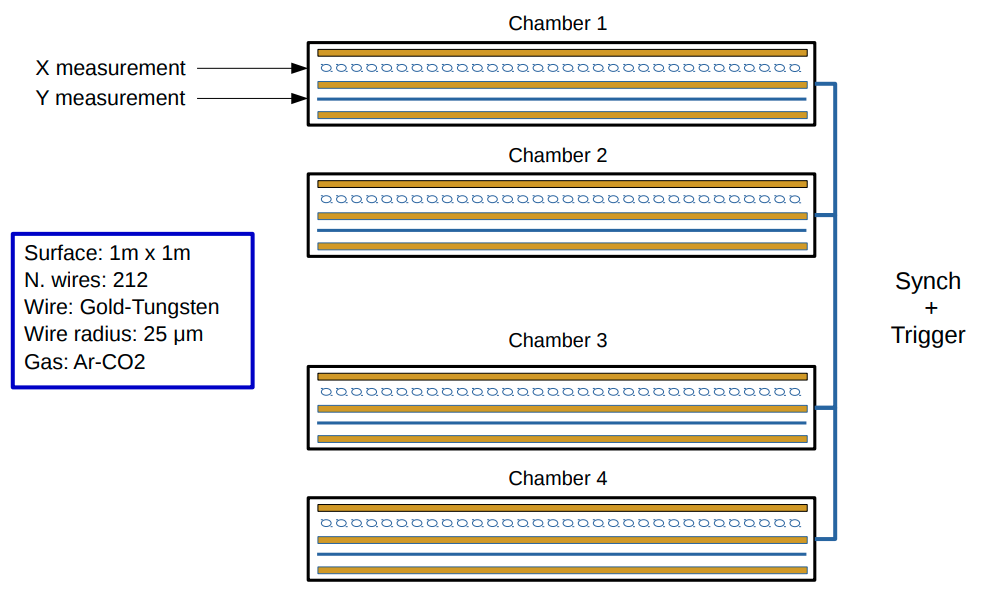
\includegraphics[width=5.5cm, height=3.7cm]{figs/muonChambers.png}
\end{minipage} \hfill
\begin{minipage}[c]{.49\textwidth}
\justifying
Quite simple experimental setup:
\begin{itemize}
\justifying
\item Two $1m^2$ detectors placed below and above the object under investigation
\item Two chambers in each detector, to measure the position and direction of muons along the x and y axes
\item Each chamber is filled with a mixture of Argon and CO$_2$
\item More than 200 wires separated by 4mm make up each chamber
\end{itemize}
\end{minipage} \hfill  \vfill

The data is collected from a USB stick and goes through a complete \textbf{\alert{reconstruction process}} before being available in a rootfile. \vfill
\end{frame}








%Statistical basis
\begin{frame}{}
\centering
	\huge{\textbf{\color{mycolor} Section II}} \newline
	\LARGE{\textbf{\color{mycolor} Statistical basis \color{black}}} \vfill
The algorithm developed heavily relies on several important statistical concepts that we can now define. \vfill
\end{frame}

\begin{frame}{Probability density functions}

\begin{minipage}[c]{.50\textwidth}
\justifying
PDFs are mathematical expressions defining probability distributions \textbf{which represent the likelihood of any given outcome}. \\ \vspace{10pt}
The area below the PDF in an interval can be interpreted as the value of the probability of a random variable occurring. 
\end{minipage}
\begin{minipage}[c]{.50\textwidth}
\begin{center}
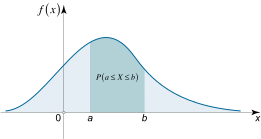
\includegraphics[width=5cm, height=2.2cm]{figs/PDF.png}
\end{center}
\end{minipage} \vfill

\begin{minipage}[c]{.50\textwidth}
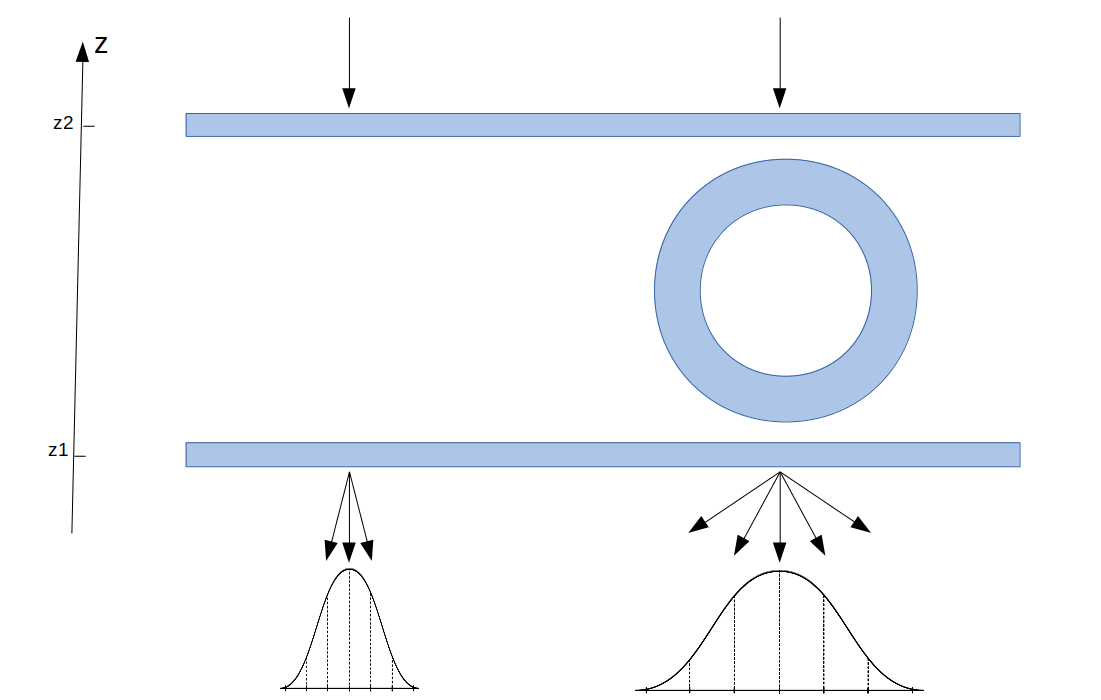
\includegraphics[width=6cm, height=3.5cm]{figs/pdfs.png}
\end{minipage}
\begin{minipage}[c]{.50\textwidth}
\justifying
The multiple scattering is a stochastic process, making PDFs extremely important. \\ \vspace{10pt} \hspace{10pt} $\rightarrow$ A thicker and denser object results in a higher expected deviation and a larger standard deviation $\sigma$ of the Gaussian PDF. 
\end{minipage}
\end{frame}

\begin{frame}{Kernel density estimation}
This method allows us to estimate the shape of an unknown PDF $f$ of a random variable $X$ from a set of $N$ observations.

\begin{minipage}[c]{.50\textwidth}
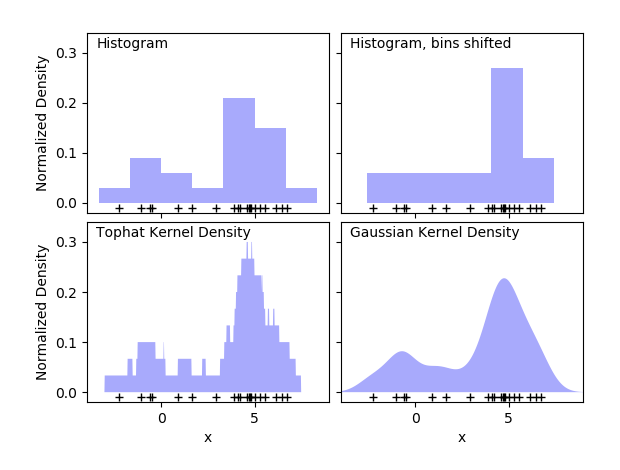
\includegraphics[width=5.8cm, height=5cm]{figs/kernels.png}
\end{minipage}
\begin{minipage}[c]{.50\textwidth}
\justifying
The usual way to proceed is to simply put the observations in an histogram, but this results in a non continous function with possible gaps. \\ \vspace{10pt}
We then define $\hat{f}_h(x)$, an estimator of $f$ defined as the sum of continous functions instead.

\begin{equation*}
\label{eq:KDF}
\hat{f}_h(x) = \frac{1}{Nh} \sum_{i=1}^{N} K \left (\frac{x-x_i}{h} \right )
\end{equation*}
\end{minipage}

Two important parameters
\begin{itemize}
\item The \textbf{\alert{kernel}} $K$, chosen as Gaussian functions in this case
\item And the \textbf{\alert{bandwidth}} $h$, a smoothing parameter.
\end{itemize} \vfill

\end{frame}

\begin{frame}{Monte-Carlo simulations}
\justifying
Monte-Carlo simulations are obtained from algorithms developed to \textbf{compute approximate numerical values to stochastic problems} using random processes and probabilistic techniques. \vfill

Instead of relying on actual data collected from the experiment, we can:
\begin{itemize}
\justifying
\item Use CRY, a cosmic ray generator to simulate thousands of incident muons
\item Make these muons go through a complete simulation of the detector done with Geant4
\item Go through the same post-processing process as actual data, \textbf{simulating thousands of experiments} without the need to perform them
\item Build the PDF for a given experiment from these simulations
\end{itemize} \vfill

Simulating an experiment is cheaper and faster than running it and allows to compare results obtained from both channels. In this work, the dependance on Geant4 will be removed as well, to make this process even faster. \vfill
\end{frame}

\begin{frame}{Maximum likelihood estimation}
\justifying
We have a way to simulate experiments, but we still need a method allowing us to reverse this process in order to \textbf{reverse this process and estimate the geometry of the object from a given measurement}. \vfill

The likelihood measures the goodness of a fit with respect to a sample of data for one or several unknown parameters. If $\bm \theta$ are the parameters of the model and $x$ is the measurement of a random variable $X$ defined from a PDF $f$, then:
\begin{equation*}
\label{eq:likelihood}
\mathcal{L}(\bm \theta | x) = f_{\bm \theta}(x) = P(X = x | \bm \theta)
\end{equation*} \vfill

The likelihood can be described as an hypersurface whose peak gives the optimal set of parameters maximizing the probability of drawing the actual sample measured. \\ \vspace{5pt}
\hspace{10pt} $\rightarrow$ The objective is then to \textbf{find the set of parameters minimizing the log-likelihood} $l(\bm \theta | x) = -2 \log(\mathcal{L}(\bm \theta | x))$. In this work, the parameter to be optimized will be the thickness of a steel pipe placed between the detectors. \vfill
\end{frame}








%The algorithm
\begin{frame}{}
\centering
	\huge{\textbf{\color{mycolor} Section III}} \newline
	\LARGE{\textbf{\color{mycolor} The algorithm \color{black}}} \vfill
Text goes here. \vfill
\end{frame}

\begin{frame}{MuonState}

\end{frame}

\begin{frame}{Surfaces and Volumes}

\end{frame}

\begin{frame}{Propagator}

\end{frame}

\begin{frame}{Likelihood}

\end{frame}












%Results obtained
\begin{frame}{}
\centering
	\huge{\textbf{\color{mycolor} Section IV}} \newline
	\LARGE{\textbf{\color{mycolor} Results obtained \color{black}}} \vfill
Text goes here. \vfill
\end{frame}

\begin{frame}{Generator validation}

\end{frame}

\begin{frame}{Pipes geometries}

\end{frame}

\begin{frame}{Kernel density functions}

\end{frame}

\begin{frame}{Likelihood curves}

\end{frame}








%Conclusions
\begin{frame}{Conclusions}

\end{frame}

\begin{frame}{Future improvements}

\end{frame}










%Back up
\begin{frame}{}
	\centering
	\huge{\textbf{\color{mycolor} Thank you  \color{black}}} \newline
	\LARGE{\textbf{\color{mycolor} for your attention! \color{black}}} \vfill

	Any questions? \vfill
\end{frame}

\appendix
	\backupbegin
	
\begin{frame}{Ionization}
\justifying
Ionization happens when the  incident muon gives some of its energy to the electrons of the absorber, as described by the Bethe-bloch formula. \vfill

\begin{equation*}
\label{eq:BB}
- \Bigl \langle \frac{dE}{dx} \Bigr \rangle = K z^2 \frac{Z}{A} \frac{1}{\beta^2} \left [\frac{1}{2} \ln \left (\frac{2 m_e c^2 \beta^2 \gamma^2 W_{\text{max}}}{I^2} - \beta^2 - \frac{\delta(\beta \gamma)}{2} \right ) \right ]
\end{equation*} \vfill

The \textbf{mass stopping power} of material depends on:
\begin{itemize}
	\item The charge number of incident particle $z$
	\item The atomic mass and charge of absorber $A$ and $Z$
	\item The relativistic factors $\beta$ and $\gamma$
	\item The maximum possible energy transfer to an electron in a single collision $W_{\text{max}}$
	\item And the mean excitation energy $I$.
\end{itemize} \vfill
\end{frame}

\begin{frame}{Ionization}
\justifying
Cosmic muons have an energy of the order of the GeV and are therefore referred to as minimum ionizing particles, so ionization is not considered in this work.
\begin{center}
	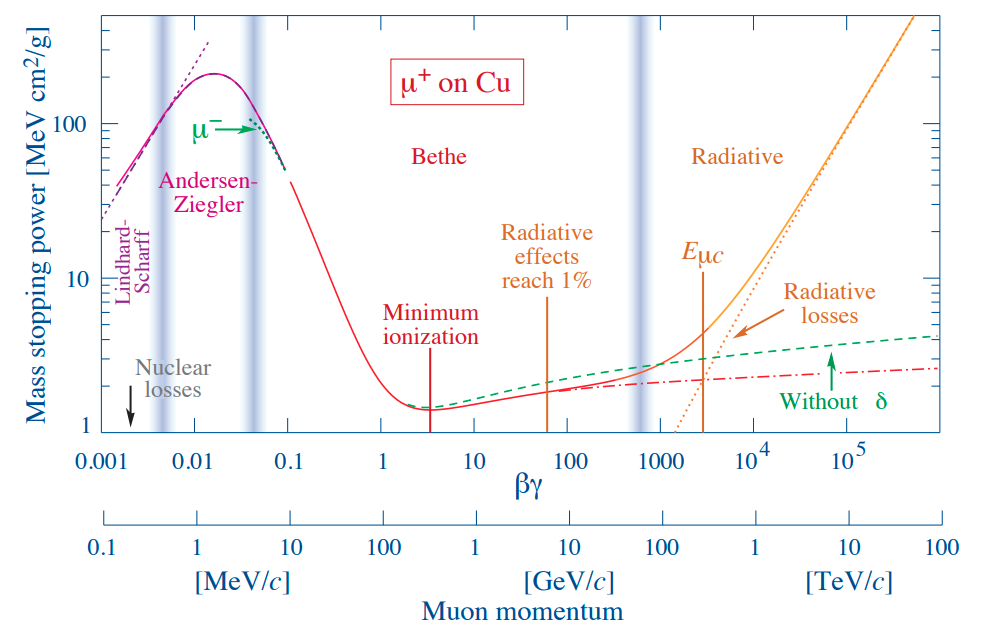
\includegraphics[width=10cm, height=6cm]{figs/BB.png}
	\end{center}
\end{frame}

\begin{frame}{Muon detectors}
\justifying
\begin{minipage}[c]{.58\textwidth}
\justifying
Multiwire proportional chambers use an array of high-voltage wires, placed within a chamber filled with a gas, in which an electric field is created. \\ \vspace{10pt}
A muon crosses the detector leaves small electric charges behind, collected by the wires while leaving a signal. The combination of the signals on the different wires give us information regarding the muon.
\end{minipage} \hfill
\begin{minipage}[c]{.39\textwidth}
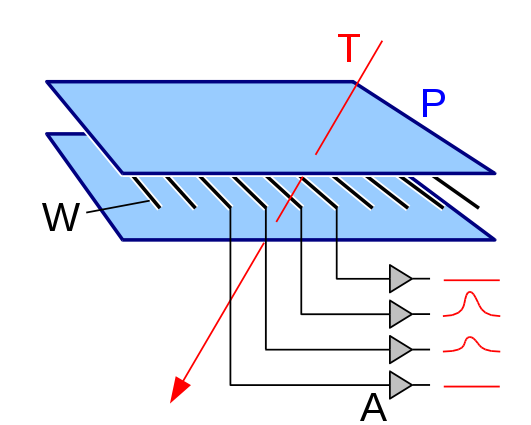
\includegraphics[width=4.2cm, height=3.5cm]{figs/wireChambers.png}
\end{minipage} \hfill \vfill

Most important parameters of a muon detector:
\begin{itemize}
\justifying
\item The \textbf{spatial resolution}, ideally as small as possible
\item The \textbf{acceptance}, related to the size of the detector
\item And the \textbf{efficiency}, which should be as high as possible to make the measurement reliable and fast.
\end{itemize}
\end{frame}

\begin{frame}{Data flow}
\begin{center}
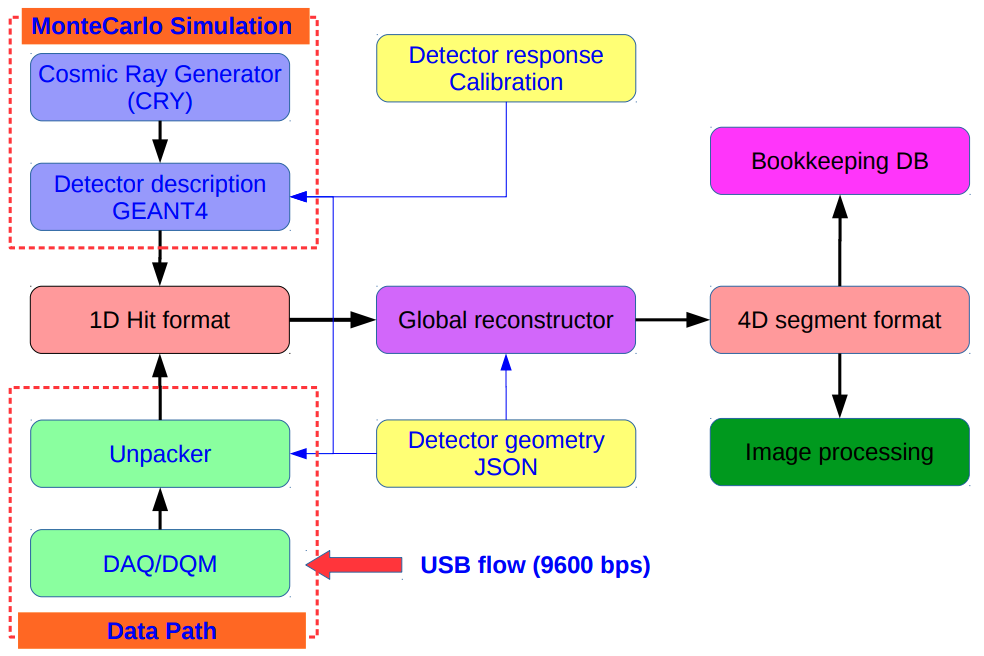
\includegraphics[width=7.5cm, height=6cm]{figs/dataFlow.png}
\end{center}
\end{frame}

\begin{frame}{Additional references}
[1] "A window into the Earth’s interior", Earthquake Research Institute,2014
\end{frame}

\backupend


 \end{document}